\documentclass[10pt,a4paper]{article}

% Core Packages
\usepackage[utf8]{inputenc}
\usepackage[T1]{fontenc}
\usepackage{lmodern}
\usepackage[margin=0.65in, top=0.75in, bottom=0.75in, headheight=14pt]{geometry}
\usepackage{amsmath,amssymb}
\usepackage{xcolor}
\usepackage{graphicx}
\usepackage{hyperref}
\usepackage{booktabs}
\usepackage{tabularx}
\usepackage{enumitem}
\usepackage{microtype}
\usepackage{titlesec}
\usepackage{parskip}
\usepackage{fancyhdr}

% TikZ and Tcolorbox for Diagrams and Highlights
\usepackage{tikz}
\usetikzlibrary{arrows.meta, positioning, shapes.geometric, shapes.misc, fit, calc, backgrounds, shadows}
\usepackage{tcolorbox}
\tcbuselibrary{skins, breakable}

% Modern Palette
\definecolor{Navy}{RGB}{15, 34, 64}
\definecolor{RoyalBlue}{RGB}{29, 78, 216}
\definecolor{Teal}{RGB}{13, 148, 136}
\definecolor{DarkGreen}{RGB}{21, 128, 61}
\definecolor{Amber}{RGB}{217, 119, 6}
\definecolor{Coral}{RGB}{225, 29, 72}
\definecolor{Purple}{RGB}{126, 34, 206}
\definecolor{Slate}{RGB}{71, 85, 105}
\definecolor{LightSlate}{RGB}{241, 245, 249}
\definecolor{SoftBlue}{RGB}{239, 246, 255}
\definecolor{SoftTeal}{RGB}{240, 253, 250}
\definecolor{SoftAmber}{RGB}{254, 252, 232}
\definecolor{SoftCoral}{RGB}{255, 241, 242}

% Geometry & Headheight
\geometry{margin=0.65in, top=0.8in, bottom=0.75in, headheight=21pt}
\addtolength{\topmargin}{-7pt}

% Hyperref Setup
\hypersetup{
    colorlinks=true,
    linkcolor=RoyalBlue,
    citecolor=Teal,
    urlcolor=RoyalBlue,
    pdftitle={Nexus Scholar Harness: A Verifiable Operating System for Academic Systematic Literature Reviews},
    pdfauthor={Nexus Scholar Team}
}

% Page Header / Footer Styling
\pagestyle{fancy}
\fancyhf{}
\renewcommand{\headrulewidth}{0.6pt}
\renewcommand{\headrule}{\hbox to\headwidth{\color{RoyalBlue!40}\leaders\hrule height \headrulewidth\hfill}}
\fancyhead[L]{\textcolor{Navy}{\textbf{Nexus Scholar Harness}} \textcolor{Slate!70}{|} \textcolor{Slate}{\small Verifiable Academic Operating System}}
\fancyhead[R]{\textcolor{Slate}{\small Supervisor Briefing \& Technical Architecture}}
\fancyfoot[L]{\textcolor{Slate!80}{\scriptsize Confidential -- Internal Academic Review \& Research Guidance}}
\fancyfoot[R]{\textcolor{Navy}{\textbf{\thepage}}}

% Section Formatting with Colored Badges and Underlines
\titleformat{\section}
  {\Large\bfseries\color{Navy}}
  {\llap{\color{RoyalBlue}\rule[-2pt]{3pt}{1.1em}\hspace{6pt}}\thesection}{0.7em}
  {\color{Navy}}
  [{\vspace{2pt}\color{RoyalBlue!30}\hrule height 0.8pt}]

\titleformat{\subsection}
  {\large\bfseries\color{RoyalBlue}}
  {\thesubsection}{0.6em}{}

\titleformat{\subsubsection}
  {\normalsize\bfseries\color{Slate}}
  {\thesubsubsection}{0.5em}{}

\titlespacing*{\section}{0pt}{10pt}{6pt}
\titlespacing*{\subsection}{0pt}{8pt}{4pt}
\titlespacing*{\subsubsection}{0pt}{6pt}{2pt}

% Custom Highlighting Badges and Pill Boxes
\newcommand{\badge}[2][RoyalBlue]{%
  \tcbox[on line, boxsep=0pt, left=4pt, right=4pt, top=2pt, bottom=2pt,
         colframe=#1, colback=#1!12, coltext=#1!80!black, arc=3pt,
         boxrule=0.6pt, fontupper=\sffamily\bfseries\tiny]{#2}%
}

\newcommand{\codebadge}[1]{%
  \tcbox[on line, boxsep=0pt, left=3pt, right=3pt, top=1.5pt, bottom=1.5pt,
         colframe=Slate!40, colback=LightSlate, coltext=Navy, arc=2pt,
         boxrule=0.5pt, fontupper=\ttfamily\scriptsize]{#1}%
}

% Custom Styled Callout Boxes
\newtcolorbox{invariantbox}[2][]{%
  enhanced,
  colback=SoftCoral,
  colframe=Coral,
  coltitle=Coral!80!black,
  fonttitle=\sffamily\bfseries\small,
  title={#2},
  boxrule=0.8pt,
  arc=4pt,
  left=8pt, right=8pt, top=6pt, bottom=6pt,
  attach boxed title to top left={xshift=10pt, yshift=-7pt},
  boxed title style={colback=SoftCoral, boxrule=0.8pt, colframe=Coral, arc=2pt},
  #1
}

\newtcolorbox{summarybox}[2][]{%
  enhanced,
  colback=SoftBlue,
  colframe=RoyalBlue,
  coltitle=Navy,
  fonttitle=\sffamily\bfseries\small,
  title={#2},
  boxrule=0.8pt,
  arc=4pt,
  left=8pt, right=8pt, top=6pt, bottom=6pt,
  attach boxed title to top left={xshift=10pt, yshift=-7pt},
  boxed title style={colback=SoftBlue, boxrule=0.8pt, colframe=RoyalBlue, arc=2pt},
  #1
}

\newtcolorbox{kitcard}[3][]{%
  enhanced,
  colback=white,
  colframe=#2!80!black,
  boxrule=0.7pt,
  arc=3pt,
  left=6pt, right=6pt, top=5pt, bottom=5pt,
  title={\textcolor{#2!90!black}{\textbf{#3}}},
  coltitle=Navy,
  fonttitle=\sffamily\footnotesize,
  colbacktitle=#2!10,
  titlerule=0.5pt,
  titlerule style=#2!40,
  #1
}

\begin{document}

% =========================================================================
% TITLE / HEADER BLOCK
% =========================================================================
\begin{tcolorbox}[enhanced, colback=Navy, colframe=Navy!90!black, arc=6pt, boxrule=0pt, left=14pt, right=14pt, top=12pt, bottom=12pt]
  \begin{minipage}{0.75\textwidth}
    {\fontsize{18}{22}\selectfont\sffamily\bfseries\textcolor{white}{Nexus Scholar Harness}}\\[3pt]
    {\large\sffamily\textcolor{Teal!25}{\textbf{A Verifiable, Deterministic Operating System for Systematic Literature Reviews}}}\\[4pt]
    {\small\sffamily\textcolor{Slate!20}{Technical Architecture, Epistemic Rigor Invariants, and Kit Ecosystem Briefing for Supervisors}}
  \end{minipage}
  \hfill
  \begin{minipage}{0.22\textwidth}
    \raggedleft
    \badge[Teal]{PRISMA 2020}\\[2pt]
    \badge[Amber]{ZERO-HALLUCINATION}\\[2pt]
    \badge[RoyalBlue]{8 SPECIALIZED KITS}\\[2pt]
    \badge[Coral]{IMMUTABLE LEDGER}
  \end{minipage}
\end{tcolorbox}

\vspace{-2pt}

% =========================================================================
% SECTION 1: INTRODUCTION & CORE PHILOSOPHY
% =========================================================================
\section{Executive Rationale: Solving the Academic AI Crisis}

Academic literature synthesis currently faces an acute reproducibility crisis. Generative Large Language Models (LLMs) frequently hallucinate citations, summarize unread abstracts rather than verified empirical sections, and obscure their reasoning inside black-box chat prompts. When conducting Systematic Literature Reviews (SLRs), Rapid Evidence Assessments (REAs), or Doctoral theses, such failure modes introduce unacceptable legal and academic liabilities.

\textbf{Nexus Scholar Harness} fundamentally inverts this paradigm. Rather than treating AI as an unconstrained author, the harness acts as a \textbf{strict, deterministic academic orchestrator}. It provides a mathematically verified substrate where autonomous agents, deterministic Python toolkits, and human Principal Investigators (PIs) collaborate under cryptographic audit guarantees.

\begin{summarybox}{Core Mission Statement}
\textbf{The Sovereign Principle:} No synthetic claim enters a research synthesis unless it satisfies an immutable $\mathbf{\ge 90\%}$ verbatim character-match threshold against verified source full-texts. The harness treats scientific evidence not as probabilistic tokens, but as a formal, verifiable state machine.
\end{summarybox}

\vspace{-2pt}

\subsection{The Three Non-Negotiable Epistemic Invariants}

\begin{itemize}[leftmargin=1.4em, itemsep=1pt, topsep=1pt]
    \item \textbf{1. Verbatim Evidence Grounding ($\ge \mathbf{90\%}$ Character Match):} Every extraction and assertion must be byte-for-byte grounded in the source PDF full-text. Fabricated conclusions and extrapolated numbers are programmatically rejected at the AST level.
    \item \textbf{2. Cryptographic Append-Only Audit Ledger (\texttt{audit/journal.jsonl}):} Every search query, multi-rater screening decision, PDF hash, and score is immutably appended to a structured JSON-Lines ledger. State can never be overwritten or erased.
    \item \textbf{3. Multi-Rater PRISMA Screening with Fleiss' $\boldsymbol{\kappa}$ Deadlock Isolation:} Screening decisions are conducted across multiple agent raters. High-agreement decisions are automated, while ambiguous papers ($<0.80$) are explicitly queued for human supervisor adjudication.
\end{itemize}

% =========================================================================
% SECTION 2: END-TO-END RESEARCH LIFECYCLE FLOW
% =========================================================================
\section{End-to-End SLR Pipeline: Flow and State Transitions}

The research process is structured into six discrete, deterministic phases. At every transition, inputs and outputs are cryptographically fingerprinted and committed to the append-only journal.

\vspace{4pt}
\begin{center}
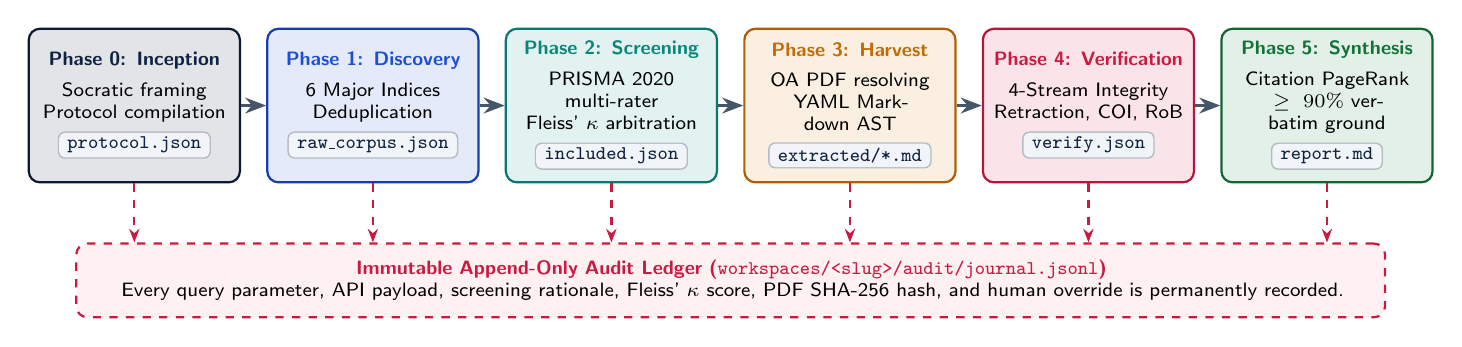
\begin{tikzpicture}[
    font=\sffamily\scriptsize,
    node distance=0.32cm,
    phase/.style={rectangle, rounded corners=4pt, draw=#1!80!black, fill=#1!12, thick, align=center, inner sep=4pt, text width=2.4cm, minimum height=1.95cm},
    auditbox/.style={rectangle, rounded corners=4pt, draw=Coral!90!black, fill=SoftCoral, dashed, thick, align=center, inner sep=6pt, text width=16.2cm},
    flowarr/.style={-{Stealth[scale=0.9]}, very thick, color=Slate},
    logarr/.style={-{Stealth[scale=0.75]}, dashed, thick, color=Coral!90!black}
]
    % Pipeline Nodes
    \node[phase=Navy] (p0) {
        \textbf{\textcolor{Navy}{Phase 0: Inception}}\\[3pt]
        Socratic framing\\
        Protocol compilation\\[3pt]
        \codebadge{protocol.json}
    };
    
    \node[phase=RoyalBlue, right=of p0] (p1) {
        \textbf{\textcolor{RoyalBlue}{Phase 1: Discovery}}\\[3pt]
        6 Major Indices\\
        Deduplication\\[3pt]
        \codebadge{raw\_corpus.json}
    };
    
    \node[phase=Teal, right=of p1] (p2) {
        \textbf{\textcolor{Teal!90!black}{Phase 2: Screening}}\\[3pt]
        PRISMA 2020 multi-rater\\
        Fleiss' $\kappa$ arbitration\\[3pt]
        \codebadge{included.json}
    };
    
    \node[phase=Amber, right=of p2] (p3) {
        \textbf{\textcolor{Amber!90!black}{Phase 3: Harvest}}\\[3pt]
        OA PDF resolving\\
        YAML Markdown AST\\[3pt]
        \codebadge{extracted/*.md}
    };
    
    \node[phase=Coral, right=of p3] (p4) {
        \textbf{\textcolor{Coral!90!black}{Phase 4: Verification}}\\[3pt]
        4-Stream Integrity\\
        Retraction, COI, RoB\\[3pt]
        \codebadge{verify.json}
    };
    
    \node[phase=DarkGreen, right=of p4] (p5) {
        \textbf{\textcolor{DarkGreen!90!black}{Phase 5: Synthesis}}\\[3pt]
        Citation PageRank\\
        $\ge 90\%$ verbatim ground\\[3pt]
        \codebadge{report.md}
    };

    % Flow Arrows
    \draw[flowarr] (p0) -- (p1);
    \draw[flowarr] (p1) -- (p2);
    \draw[flowarr] (p2) -- (p3);
    \draw[flowarr] (p3) -- (p4);
    \draw[flowarr] (p4) -- (p5);

    % Audit Ledger anchored safely below the phase boxes
    \node[auditbox, below=0.75cm of $(p2.south)!0.5!(p3.south)$] (audit) {
        \textbf{\textcolor{Coral!90!black}{Immutable Append-Only Audit Ledger (\texttt{workspaces/<slug>/audit/journal.jsonl})}}\\
        \scriptsize Every query parameter, API payload, screening rationale, Fleiss' $\kappa$ score, PDF SHA-256 hash, and human override is permanently recorded.
    };

    % Audit logging connections
    \draw[logarr] (p0.south) -- (p0.south |- audit.north);
    \draw[logarr] (p1.south) -- (p1.south |- audit.north);
    \draw[logarr] (p2.south) -- (p2.south |- audit.north);
    \draw[logarr] (p3.south) -- (p3.south |- audit.north);
    \draw[logarr] (p4.south) -- (p4.south |- audit.north);
    \draw[logarr] (p5.south) -- (p5.south |- audit.north);

\end{tikzpicture}
\end{center}
\vspace{-4pt}

\newpage
% =========================================================================
% SECTION 3: SYSTEM ARCHITECTURE & THE 8 KITS
% =========================================================================
\section{System Architecture: Thin Orchestrator \& Decoupled Toolkits}

A critical architectural virtue of the Nexus Scholar Harness is that it is \textbf{strictly decoupled}. The harness contains zero domain logic; it is a thin orchestrator that delegates execution to eight specialized, editable Python toolkits located under \codebadge{tools/<kit>/}. These kits function both as high-performance CLI tools and as modular libraries exposed to AI agents via the \textbf{Model Context Protocol (MCP)}.

\vspace{4pt}
\begin{center}
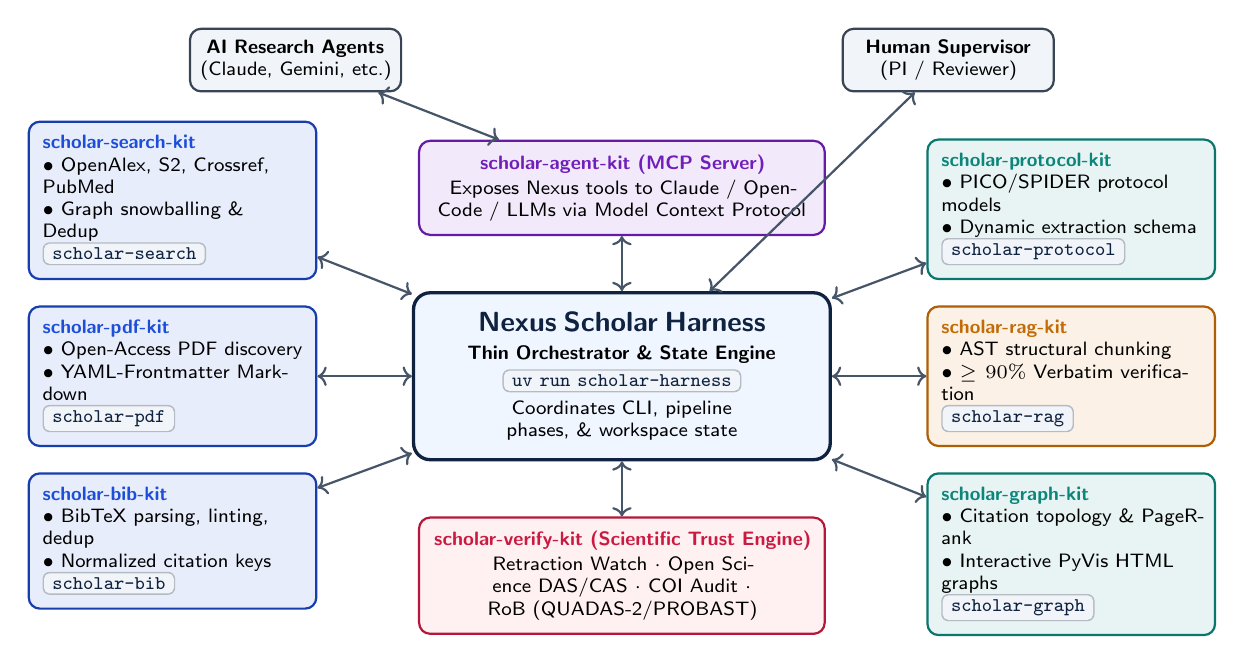
\begin{tikzpicture}[
    font=\sffamily\scriptsize,
    node distance=1.1cm and 1.3cm,
    core/.style={rectangle, rounded corners=6pt, draw=Navy, fill=SoftBlue, very thick, align=center, inner sep=7pt, text width=4.8cm},
    kitnode/.style={rectangle, rounded corners=4pt, draw=#1!80!black, fill=#1!10, thick, align=left, inner sep=5pt, text width=3.3cm},
    mcpnode/.style={rectangle, rounded corners=4pt, draw=Purple!80!black, fill=Purple!10, thick, align=center, inner sep=5pt, text width=4.8cm},
    verifnode/.style={rectangle, rounded corners=4pt, draw=Coral!80!black, fill=SoftCoral, thick, align=center, inner sep=5pt, text width=4.8cm},
    actor/.style={rectangle, rounded corners=4pt, draw=Slate!80!black, fill=LightSlate, thick, align=center, inner sep=4pt, text width=2.4cm},
    arr/.style={-{Stealth[scale=0.85]}, thick, color=Slate}
]
    % Core Orchestrator
    \node[core] (orch) {
        \textbf{\normalsize\textcolor{Navy}{Nexus Scholar Harness}}\\[2pt]
        \textbf{Thin Orchestrator \& State Engine}\\[2pt]
        \codebadge{uv run scholar-harness}\\[2pt]
        \scriptsize Coordinates CLI, pipeline phases, \& workspace state
    };

    % Left Tier: Ingestion & Discovery
    \node[kitnode=RoyalBlue, left=1.2cm of orch] (pdf) {
        \textbf{\textcolor{RoyalBlue}{scholar-pdf-kit}}\\
        $\bullet$ Open-Access PDF discovery\\
        $\bullet$ YAML-Frontmatter Markdown\\
        \codebadge{scholar-pdf}
    };
    \node[kitnode=RoyalBlue, above=0.32cm of pdf] (search) {
        \textbf{\textcolor{RoyalBlue}{scholar-search-kit}}\\
        $\bullet$ OpenAlex, S2, Crossref, PubMed\\
        $\bullet$ Graph snowballing \& Dedup\\
        \codebadge{scholar-search}
    };
    \node[kitnode=RoyalBlue, below=0.32cm of pdf] (bib) {
        \textbf{\textcolor{RoyalBlue}{scholar-bib-kit}}\\
        $\bullet$ BibTeX parsing, linting, dedup\\
        $\bullet$ Normalized citation keys\\
        \codebadge{scholar-bib}
    };

    % Right Tier: Rigor & Cognitive Processing
    \node[kitnode=Amber, right=1.2cm of orch] (rag) {
        \textbf{\textcolor{Amber!90!black}{scholar-rag-kit}}\\
        $\bullet$ AST structural chunking\\
        $\bullet$ $\ge 90\%$ Verbatim verification\\
        \codebadge{scholar-rag}
    };
    \node[kitnode=Teal, above=0.32cm of rag] (proto) {
        \textbf{\textcolor{Teal!90!black}{scholar-protocol-kit}}\\
        $\bullet$ PICO/SPIDER protocol models\\
        $\bullet$ Dynamic extraction schema\\
        \codebadge{scholar-protocol}
    };
    \node[kitnode=Teal, below=0.32cm of rag] (graph) {
        \textbf{\textcolor{Teal!90!black}{scholar-graph-kit}}\\
        $\bullet$ Citation topology \& PageRank\\
        $\bullet$ Interactive PyVis HTML graphs\\
        \codebadge{scholar-graph}
    };

    % Top: Agent Interface (MCP)
    \node[mcpnode, above=0.7cm of orch] (agent) {
        \textbf{\textcolor{Purple!90!black}{scholar-agent-kit (MCP Server)}}\\[1pt]
        Exposes Nexus tools to Claude / OpenCode / LLMs via Model Context Protocol
    };

    % Bottom: Verification Suite
    \node[verifnode, below=0.7cm of orch] (verify) {
        \textbf{\textcolor{Coral!90!black}{scholar-verify-kit (Scientific Trust Engine)}}\\[1pt]
        Retraction Watch $\cdot$ Open Science DAS/CAS $\cdot$ COI Audit $\cdot$ RoB (QUADAS-2/PROBAST)
    };

    % External Actors
    \node[actor, above left=0.6cm and 0.2cm of agent] (llm) {\textbf{AI Research Agents}\\(Claude, Gemini, etc.)};
    \node[actor, above right=0.6cm and 0.2cm of agent] (pi) {\textbf{Human Supervisor}\\(PI / Reviewer)};

    % Actor connections
    \draw[arr, <->] (llm) -- (agent);
    \draw[arr, <->] (pi) -- (orch);

    % Orchestrator to Kits
    \draw[arr, <->] (orch) -- (search);
    \draw[arr, <->] (orch) -- (pdf);
    \draw[arr, <->] (orch) -- (bib);
    \draw[arr, <->] (orch) -- (proto);
    \draw[arr, <->] (orch) -- (rag);
    \draw[arr, <->] (orch) -- (graph);
    \draw[arr, <->] (orch) -- (agent);
    \draw[arr, <->] (orch) -- (verify);

\end{tikzpicture}
\end{center}
\vspace{-4pt}

\subsection{Detailed Breakdown of the 8 Specialized Toolkits}

\begin{enumerate}[leftmargin=1.4em, itemsep=2.5pt, topsep=2pt]
    \item \textbf{\texttt{scholar-search-kit}} \badge[RoyalBlue]{Discovery \& Screening}: Connects directly to OpenAlex, Semantic Scholar, Crossref, PubMed, arXiv, and bioRxiv. Performs algorithmic deduplication (DOI, fuzzy title matching) and iterative citation snowballing. Emits structured PRISMA corpus files. \hfill \textit{Doc: \href{https://github.com/nexus-scholar/nexus-scholar-harness/blob/main/tools/scholar-search-kit/README.md}{\codebadge{tools/scholar-search-kit}}}
    
    \item \textbf{\texttt{scholar-pdf-kit}} \badge[RoyalBlue]{Harvest \& Extraction}: Resolves Open Access PDF locations, verifies document integrity, and extracts PDF contents into structured Markdown with standardized YAML frontmatter metadata. Eliminates PDF formatting artifacts. \hfill \textit{Doc: \href{https://github.com/nexus-scholar/nexus-scholar-harness/blob/main/tools/scholar-pdf-kit/README.md}{\codebadge{tools/scholar-pdf-kit}}}
    
    \item \textbf{\texttt{scholar-bib-kit}} \badge[RoyalBlue]{Bibliography Curation}: Parses, normalizes, lints, and merges BibTeX databases. Enforces canonical citation keys and standardizes journal naming conventions across heterogeneous sources. \hfill \textit{Doc: \href{https://github.com/nexus-scholar/nexus-scholar-harness/blob/main/tools/scholar-bib-kit/README.md}{\codebadge{tools/scholar-bib-kit}}}
    
    \item \textbf{\texttt{scholar-protocol-kit}} \badge[Teal]{Methodological Framework}: Formulates, validates, and mathematically fingerprints research protocols. Generates dynamic extraction models based on PICO, SPIDER, or custom criteria, guaranteeing adherence to study boundaries. \hfill \textit{Doc: \href{https://github.com/nexus-scholar/nexus-scholar-harness/blob/main/tools/scholar-protocol-kit/README.md}{\codebadge{tools/scholar-protocol-kit}}}
    
    \item \textbf{\texttt{scholar-verify-kit}} \badge[Coral]{Trust \& Integrity}: Audits the literature corpus across four critical dimensions: (1) Retraction checking via Crossref/OpenAlex, (2) Open-Science compliance scanning (Data and Code Availability Statements), (3) Conflict of Interest (COI) disclosures, and (4) QUADAS-2 and PROBAST Risk-of-Bias (RoB) scores. \hfill \textit{Doc: \href{https://github.com/nexus-scholar/nexus-scholar-harness/blob/main/tools/scholar-verify-kit/README.md}{\codebadge{tools/scholar-verify-kit}}}
    
    \item \textbf{\texttt{scholar-rag-kit}} \badge[Amber]{AST Chunking \& Grounded RAG}: Parses full-text Markdown into Abstract Syntax Trees (ASTs), preserving section hierarchies (Methods, Results, Limitations). Powers hybrid graph-boosted vector retrieval with strict verbatim verification. \hfill \textit{Doc: \href{https://github.com/nexus-scholar/nexus-scholar-harness/blob/main/tools/scholar-rag-kit/README.md}{\codebadge{tools/scholar-rag-kit}}}
    
    \item \textbf{\texttt{scholar-graph-kit}} \badge[Teal]{Citation Networks}: Builds multi-directional citation graphs, computes normalized PageRank to identify landmark foundational papers, and generates interactive PyVis HTML visual network diagrams. \hfill \textit{Doc: \href{https://github.com/nexus-scholar/nexus-scholar-harness/blob/main/tools/scholar-graph-kit/README.md}{\codebadge{tools/scholar-graph-kit}}}
    
    \item \textbf{\texttt{scholar-agent-kit}} \badge[Purple]{Model Context Protocol (MCP)}: Implements an official MCP server exposing all seven underlying deterministic toolkits as structured tools to AI agent runtimes (Claude Desktop, OpenCode, Gemini). \hfill \textit{Doc: \href{https://github.com/nexus-scholar/nexus-scholar-harness/blob/main/tools/scholar-agent-kit/README.md}{\codebadge{tools/scholar-agent-kit}}}
\end{enumerate}

\newpage
% =========================================================================
% SECTION 4: AGENT-IN-THE-LOOP SCREENING SEQUENCE
% =========================================================================
\section{Agent-in-the-Loop Screening: Interaction Sequence}

A key differentiator of the Nexus Scholar Harness is its \textbf{agent-in-the-loop file handoff} architecture for PRISMA screening. Unlike naive implementations that send thousands of abstracts through opaque prompt chains, the harness splits the screening workload into discrete, audit-tracked batches. AI agents independently screen the batches, calculate statistical agreement, and automatically escalate contentious papers to the human supervisor.

\vspace{6pt}
\begin{center}
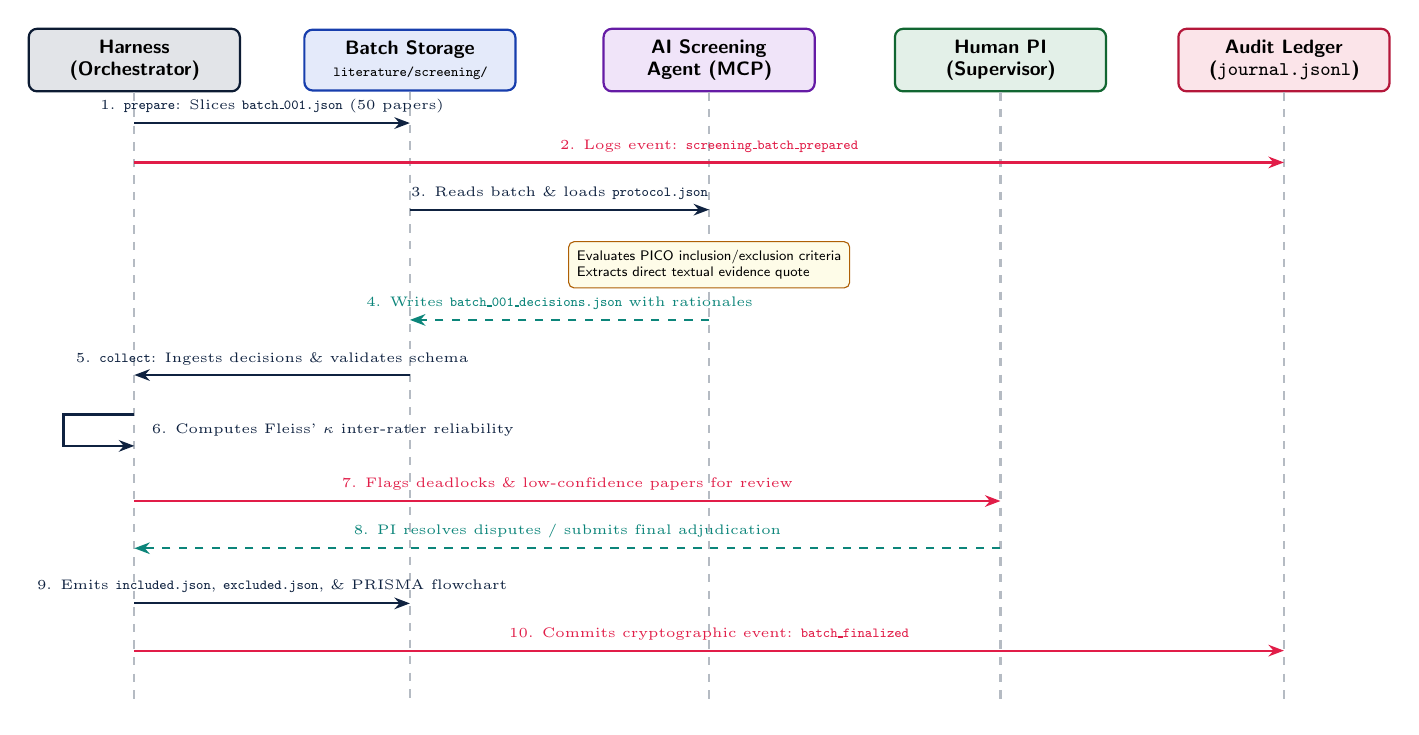
\begin{tikzpicture}[
    font=\sffamily\scriptsize,
    lifeline/.style={draw=Slate!40, dashed, thick},
    entity/.style={rectangle, rounded corners=3pt, draw=#1!80!black, fill=#1!12, thick, align=center, inner sep=4pt, text width=2.4cm, font=\sffamily\bfseries\scriptsize},
    msg/.style={-{Stealth[scale=0.85]}, thick, color=Navy},
    reply/.style={-{Stealth[scale=0.85]}, dashed, thick, color=Teal!90!black},
    alert/.style={-{Stealth[scale=0.85]}, thick, color=Coral},
    note/.style={rectangle, rounded corners=2pt, draw=Amber!80!black, fill=SoftAmber, align=left, inner sep=3pt, font=\sffamily\tiny}
]
    % Lifeline Headers
    \node[entity=Navy] (orch) at (0, 0) {Harness\\(Orchestrator)};
    \node[entity=RoyalBlue] (disk) at (3.5, 0) {Batch Storage\\\texttt{\tiny literature/screening/}};
    \node[entity=Purple] (agent) at (7.3, 0) {AI Screening\\Agent (MCP)};
    \node[entity=DarkGreen] (pi) at (11.0, 0) {Human PI\\(Supervisor)};
    \node[entity=Coral] (audit) at (14.6, 0) {Audit Ledger\\(\texttt{journal.jsonl})};

    % Vertical Lifelines
    \draw[lifeline] (orch) -- (0, -8.2);
    \draw[lifeline] (disk) -- (3.5, -8.2);
    \draw[lifeline] (agent) -- (7.3, -8.2);
    \draw[lifeline] (pi) -- (11.0, -8.2);
    \draw[lifeline] (audit) -- (14.6, -8.2);

    % Sequence steps
    % Step 1: Prepare
    \draw[msg] (0, -0.8) -- node[above, font=\tiny] {1. \texttt{prepare}: Slices \texttt{batch\_001.json} (50 papers)} (3.5, -0.8);
    \draw[alert] (0, -1.3) -- node[above, font=\tiny] {2. Logs event: \texttt{screening\_batch\_prepared}} (14.6, -1.3);

    % Step 2: Agent reads batch
    \draw[msg] (3.5, -1.9) -- node[above, font=\tiny] {3. Reads batch \& loads \texttt{protocol.json}} (7.3, -1.9);
    \node[note] at (7.3, -2.6) {Evaluates PICO inclusion/exclusion criteria\\Extracts direct textual evidence quote};

    % Step 3: Agent writes decisions
    \draw[reply] (7.3, -3.3) -- node[above, font=\tiny] {4. Writes \texttt{batch\_001\_decisions.json} with rationales} (3.5, -3.3);

    % Step 4: Collect & Agreement
    \draw[msg] (3.5, -4.0) -- node[above, font=\tiny] {5. \texttt{collect}: Ingests decisions \& validates schema} (0, -4.0);
    \draw[msg] (0, -4.5) -- (-0.9, -4.5) -- (-0.9, -4.9) -- (0, -4.9);
    \node[anchor=west, font=\tiny, Navy] at (0.1, -4.7) {6. Computes Fleiss' $\kappa$ inter-rater reliability};

    % Step 5: Disagreement / Adjudication
    \draw[alert] (0, -5.6) -- node[above, font=\tiny] {7. Flags deadlocks \& low-confidence papers for review} (11.0, -5.6);
    \draw[reply] (11.0, -6.2) -- node[above, font=\tiny] {8. PI resolves disputes / submits final adjudication} (0, -6.2);

    % Step 6: Final Output & Commit
    \draw[msg] (0, -6.9) -- node[above, font=\tiny] {9. Emits \texttt{included.json}, \texttt{excluded.json}, \& PRISMA flowchart} (3.5, -6.9);
    \draw[alert] (0, -7.5) -- node[above, font=\tiny] {10. Commits cryptographic event: \texttt{batch\_finalized}} (14.6, -7.5);

\end{tikzpicture}
\end{center}
\vspace{-4pt}

\subsection{Why the Agent-in-the-Loop Pattern Outperforms Direct LLM Prompting}

\begin{itemize}[leftmargin=1.4em, itemsep=1.5pt, topsep=1pt]
    \item \textbf{Decoupled Execution:} The orchestrator stops after writing each batch file. Screening agents can run asynchronously, in parallel, across local LLMs (e.g. Ollama) or proprietary frontier APIs without blocking the main workflow.
    \item \textbf{Statistical Rigor (Fleiss' $\boldsymbol{\kappa}$):} Screening reliability is quantified mathematically rather than assumed. If raters disagree, the harness refuses to guess, quarantining the ambiguous candidate for supervisor intervention.
    \item \textbf{Audited Human Adjudication:} The supervisor's decisions are explicitly preserved in the audit log alongside the agent's initial rationale, providing complete defense in peer-reviewed methodology sections.
\end{itemize}

% =========================================================================
% SECTION 5: SUPERVISOR VALUE PROPOSITION
% =========================================================================
\section{Strategic Value for Supervisors and Research Labs}

\begin{invariantbox}{Why Nexus Scholar Harness Protects the Lab's Reputation}
\begin{itemize}[leftmargin=1.2em, itemsep=1.5pt, topsep=1pt]
    \item \textbf{Immunity Against Retraction Scandals:} \texttt{scholar-verify-kit} automatically identifies retracted papers or expressions of concern before they can contaminate literature reviews.
    \item \textbf{Verifiable $\ge \mathbf{90\%}$ Quotation Grounding:} Eliminates the threat of fabricated findings in student-authored reviews. Every quantitative claim links directly to character offsets in source PDFs.
    \item \textbf{Submission-Ready PRISMA 2020 Artifacts:} Generates publication-grade PRISMA flowcharts, data extraction matrices, and BibTeX databases ready for submission to high-impact journals (e.g., Nature, IEEE, ACM, Lancet).
    \item \textbf{Complete Reproducibility for Doctoral Defenses:} The entire review lifecycle can be replayed and verified from \codebadge{audit/journal.jsonl} by peer reviewers, examiners, and grant committees.
\end{itemize}
\end{invariantbox}

\newpage
% =========================================================================
% SECTION 6: MASTER SPECIFICATION & REFERENCE MATRIX
% =========================================================================
\section{Master Reference Matrix: Ecosystem Toolkits \& Documentation}

Every toolkit in the Nexus Scholar ecosystem is individually tracked, test-covered, and documented. The table below serves as the definitive reference for library capabilities, CLI entrypoints, MCP tools, and technical documentation links.

\vspace{4pt}
\begin{center}
\small
\renewcommand{\arraystretch}{1.25}
\begin{tabularx}{\textwidth}{@{} l >{\raggedright\arraybackslash}X >{\raggedright\arraybackslash}p{3.3cm} >{\raggedright\arraybackslash}p{3.6cm} @{}}
\toprule
\textbf{\textcolor{Navy}{Toolkit}} & \textbf{\textcolor{Navy}{Primary Function}} & \textbf{\textcolor{Navy}{CLI Entrypoint}} & \textbf{\textcolor{Navy}{Documentation \& Surface}} \\
\midrule
\textbf{\texttt{scholar-harness}} & Core orchestrator, state machine, CLI wizard, project workspace manager & \codebadge{uv run scholar-harness} & \href{https://github.com/nexus-scholar/nexus-scholar-harness/blob/main/docs/kits_surface_matrix.md}{\codebadge{docs/kits\_surface\_matrix.md}} \\

\textbf{\texttt{scholar-search-kit}} & Multi-index API discovery, fuzzy deduplication, citation snowballing & \codebadge{scholar-search} & \href{https://github.com/nexus-scholar/nexus-scholar-harness/blob/main/tools/scholar-search-kit/README.md}{\codebadge{tools/scholar-search-kit/}} \\

\textbf{\texttt{scholar-pdf-kit}} & Open Access PDF resolver, integrity validator, structural YAML-Markdown & \codebadge{scholar-pdf} & \href{https://github.com/nexus-scholar/nexus-scholar-harness/blob/main/tools/scholar-pdf-kit/README.md}{\codebadge{tools/scholar-pdf-kit/}} \\

\textbf{\texttt{scholar-bib-kit}} & BibTeX parsing, schema linting, deduplication, citation key formatting & \codebadge{scholar-bib} & \href{https://github.com/nexus-scholar/nexus-scholar-harness/blob/main/tools/scholar-bib-kit/README.md}{\codebadge{tools/scholar-bib-kit/}} \\

\textbf{\texttt{scholar-protocol-kit}} & Research protocol compilation, criteria validation, schema fingerprinting & \codebadge{scholar-protocol} & \href{https://github.com/nexus-scholar/nexus-scholar-harness/blob/main/tools/scholar-protocol-kit/README.md}{\codebadge{tools/scholar-protocol-kit/}} \\

\textbf{\texttt{scholar-verify-kit}} & 4-stream trust audit: Retractions, DAS/CAS scanning, COI, RoB & \codebadge{scholar-verify} & \href{https://github.com/nexus-scholar/nexus-scholar-harness/blob/main/tools/scholar-verify-kit/README.md}{\codebadge{tools/scholar-verify-kit/}} \\

\textbf{\texttt{scholar-rag-kit}} & AST section-aware chunking, hybrid vector retrieval, $\ge 90\%$ grounding & \codebadge{scholar-rag} & \href{https://github.com/nexus-scholar/nexus-scholar-harness/blob/main/tools/scholar-rag-kit/README.md}{\codebadge{tools/scholar-rag-kit/}} \\

\textbf{\texttt{scholar-graph-kit}} & Citation network topology, PageRank score ranking, PyVis HTML rendering & \codebadge{scholar-graph} & \href{https://github.com/nexus-scholar/nexus-scholar-harness/blob/main/tools/scholar-graph-kit/README.md}{\codebadge{tools/scholar-graph-kit/}} \\

\textbf{\texttt{scholar-agent-kit}} & Model Context Protocol (MCP) server bridging agents to Nexus tools & \codebadge{uv run scholar-agent} & \href{https://github.com/nexus-scholar/nexus-scholar-harness/blob/main/tools/scholar-agent-kit/README.md}{\codebadge{tools/scholar-agent-kit/}} \\
\bottomrule
\end{tabularx}
\end{center}

\vspace{4pt}

\begin{summarybox}{Paradigm Comparison: Nexus Scholar Harness vs. Commercial AI Tools}
\footnotesize
\begin{itemize}[leftmargin=1.2em, itemsep=1.5pt, topsep=1pt]
    \item \textbf{Verbatim Character Grounding:} Commercial LLMs summarize abstracts with hallucination risks; Nexus enforces a $\ge 90\%$ byte-level quotation match against source full-texts.
    \item \textbf{PRISMA 2020 Compliance:} Nexus implements multi-rater batch screening with Fleiss' $\kappa$ arbitration and supervisor deadlock escalation, whereas commercial tools operate as un-auditable single-prompt queries.
    \item \textbf{Scientific Trust \& Integrity:} Nexus provides automated 4-stream verification (retraction alerts, DAS/CAS artifact scanning, COI audits, and deterministic QUADAS-2/PROBAST risk-of-bias scores).
    \item \textbf{Local-First Data Sovereignty:} All code, queries, full-texts, and audit traces reside locally under \codebadge{workspaces/<slug>/}, git-versioned and immune to external platform API shutdowns or proprietary lock-in.
\end{itemize}
\end{summarybox}

\vspace{4pt}

\section{Summary and Recommended Next Steps}

The Nexus Scholar Harness provides your research group with an enterprise-grade, scientifically rigorous framework that transforms the traditional, error-prone literature review process into a fully reproducible, mathematically verified computational workflow. 

\begin{tcolorbox}[enhanced, colback=SoftTeal, colframe=Teal, arc=4pt, boxrule=0.8pt, left=10pt, right=10pt, top=8pt, bottom=8pt]
\sffamily\textbf{\textcolor{Teal!90!black}{Recommended Protocol for Supervisor / Student Implementation:}}
\begin{enumerate}[leftmargin=1.4em, itemsep=2pt, topsep=2pt]
    \item \textbf{Initialize Workspace:} Execute \codebadge{uv run scholar-harness inception} to launch the conversational Phase-0 wizard and formulate \codebadge{protocol.json} with explicit PICO/SPIDER boundaries.
    \item \textbf{Execute Search \& Deduplication:} Run the automated discovery phase across all six databases to assemble the baseline corpus in \codebadge{literature/raw\_corpus.json}.
    \item \textbf{Conduct Supervised PRISMA Screening:} Launch the batch agent screening process via \codebadge{python src/scholar\_harness/agent\_screen.py prepare}. Review any flagged deadlock candidates where Fleiss' $\kappa < 0.80$.
    \item \textbf{Verify Integrity \& Synthesize:} Execute the 4-stream verification audit via \codebadge{uv run scholar-verify} and inspect the generated PyVis citation network and grounded synthesis report.
\end{enumerate}
\end{tcolorbox}

\vspace{6pt}
\begin{center}
\textcolor{Slate!70}{\footnotesize $\blacksquare$ Document prepared for academic supervisor review $\cdot$ Source repository: \href{https://github.com/nexus-scholar/nexus-scholar-harness}{\codebadge{nexus-scholar-harness}} $\blacksquare$}
\end{center}

\end{document}
